\documentclass[12pt,a4paper,twoside]{article}
\usepackage[utf8]{inputenc}
\usepackage[spanish]{babel}
\usepackage{amsmath}
\usepackage{amsfonts}
\usepackage{amssymb}
\usepackage{graphicx}
\usepackage[left=2cm,right=2cm,top=2cm,bottom=2cm]{geometry}
\usepackage{lmodern}
\usepackage{textcomp}
\author{Yoleivys Delgado}
\title{\textbf{Movimiento de Proyectil}}

\begin{document}
\maketitle
El movimiento de proyectil es una forma de movimiento donde un cuerpo o partícula es lanzado cerca de la superficie terrestre y adquiere un movimiento a lo largo de una trayectoria parabólica bajo la acción de la gravedad. En este tipo de movimiento se considera la resistencia con el aire despreciable.

\section*{Ejemplo: Movimientos de proyectil usando Fortran}
Realiza las gráficas de la trayectoria de un proyectil que es lanzado con una rapidez inicial de $10\hspace{0.2cm}m/s$, con ángulos iniciales de $ 15^{\circ}, 30^{\circ}, 45^{\circ}, 60^{\circ}, 75^{\circ}$  y $ 90^{\circ}$.
\vspace{0.5cm}

Para la realización de este ejercicio se utilizaran las  ecuaciones 1 y 2, las cuales me permiten determinar el desplazamiento horizontal y vertical en cualquier instante de tiempo. Los intervalos de tiempos elegidos fueron fracciones del tiempo de vuelo, el cual fue determinado usando la ecuación 3. 

\begin{eqnarray}
x = v_{0} t cos (\theta)\\
y = v_{0} t sin (\theta) - \frac{1}{2} g t^2\\
t = \frac{2v_{0}sin (\theta)}{g}
\end{eqnarray}

En la realización de las gráficas de los proyectiles tomamos 20 puntos, es decir, 20 tiempos diferentes para cada uno de los ángulos. En la figura (\ref{fig:figura1}) se muestra la gráfica obtenida de la trayectoria de los proyectiles lanzados a los ángulos de $ 15^{\circ}, 30^{\circ}, 45^{\circ}, 60^{\circ}, 75^{\circ}$  y $ 90^{\circ}$.
\newpage   
\begin{figure}[h]
\centering
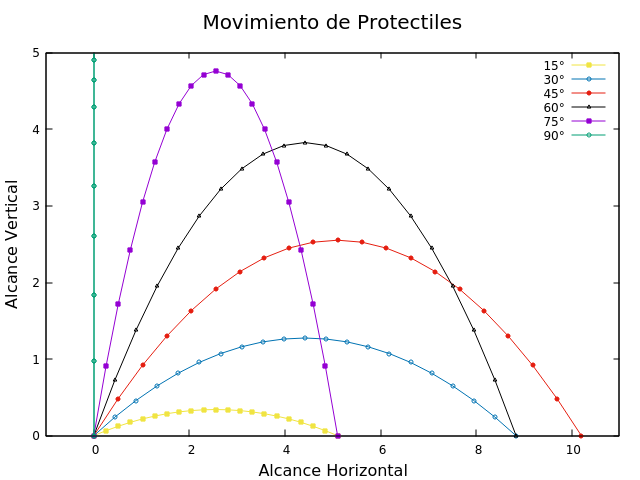
\includegraphics[width=10cm]{proyectiles.png} 
\caption{Trayectorias seguida por un proyectil lanzados a diferentes ángulos}
\label{fig:figura1}
\end{figure}

los códigos de gnuplot y fortran utilizados para la realización del ejercicio y graficación del mismo se presentan en la figura (\ref{fig:figura2}) y figura (\ref{fig:figura3})
\vspace{0.5cm}

\begin{figure}[h]
 \centering 
\begin{verbatim}
set title 'Movimiento de Proyectiles'
set title font ",15" norotate
set xlabel "Alcance Horizontal"
set xlabel font "Verdana,12"
set ylabel "Alcance Vertical"
set ylabel font "Verdana,12"
set style data points
set xrange [-1:11]
set yrange [0:5]
set pointsize 0.7
plot "datos.dat" index 0 using 1:2  with linespoints ls 5 title "15°",\
"datos.dat" index 1 using 1:2  with linespoints ls 6 title "$30°",\
"datos.dat" index 2 using 1:2  with linespoints ls 7 title "45°",\
"datos.dat" index 3 using 1:2  with linespoints ls 8 title "60°",\
"datos.dat" index 4 using 1:2  with linespoints ls 9 title "75°",\
"datos.dat" index 5 using 1:2  with linespoints ls 10 title "90°"
\end{verbatim}

\caption{Codigo gnuplot de la grafica de la figura 1}
\label{fig:figura2}
\end{figure}

\begin{figure}[h]
 \centering
\begin{verbatim}
program desplazamientos

  implicit none

  ! definimos constantes
  real, parameter :: g = 9.8, pi =3.1415
  real, dimension (20) :: t=0., x=0., y=0.
  real ::tv, a, v0
  integer :: i, j, npoints
  
  write(*,*) ' Movimiento de Proyectiles'
  write(*,*) 'Escribe la rapidez inicial y el numero de puntos'
  read(*,*)  v0, npoints

  loopangulo: do j=15,90,15
    ! convirtiendo ángulo a radianes
     a = j * pi / 180.0

  ! la ecuacion de tiempo de vuelo es
     tv = (2 * v0 * sin(a))/ g
     
     loopposicion: do i= 0, npoints
     t(i) =t(i)+ i * (tv /real(npoints))
     x(i) =x(i)+ v0 * t(i) * cos (a)
     y(i) =  y(i)+ (2* v0 * t(i) * sin (a) - g* t(i)**2 )/ 2
     open (1, file = 'datos.dat', status= 'unknown')
     write(1,1000)  x(i), y(i)
     1000 format (F15.10, 5x, F15.10)
     
  end do loopposicion
  write (1,1100)
     1100 format (//)
  do i = 0,npoints
     t(i)=0
     x(i)=0
     y(i)=0
  end do
 
end do loopangulo

close (1)
end program desplazamientos
\end{verbatim}
\caption{Programa Fortran del calculo de las posiciones horizontal y vertical seguida por un proyectil a diferentes ángulos}
\label{fig:figura3} 
\end{figure}


\end{document}